%!TEX program = xelatex
%% Copyright (C) 2025 傅祉珏
%% 
%% This file contains LaTeX source code for the Homework3 of YatRL,
%% released under AGPLv3 license.
%% Full license text available in LICENSE file at project root,
%% with additional restrictions in ADDITIONAL_TERMS.md.
%% 
%% Commercial use prohibited. Academic use requires retention of this notice.
%% Source repository: https://github.com/Billiefu/YatRL

% SPDX-FileCopyrightText: 2025 傅祉珏
% SPDX-License-Identifier: AGPL-3.0-or-later
% SPDX-Additional-Clauses: see ADDITIONAL_TERMS.md

\documentclass[a4paper, utf8]{ctexart}
\usepackage[fontset=Fandol]{ctex}
\usepackage{draftwatermark}
\usepackage{algpseudocode}
\usepackage{algorithmicx}
\usepackage{anyfontsize}
\usepackage{subcaption}
\usepackage{algorithm}
\usepackage{abstract}
\usepackage{amsfonts}
\usepackage{appendix}
\usepackage{enumitem}
\usepackage{fancyhdr}
\usepackage{fontspec}
\usepackage{geometry}
\usepackage{graphicx}
\usepackage{amsmath}
\usepackage{caption}
\usepackage{lipsum}
\usepackage{minted}
\usepackage{url}

\usepackage{tikz}
\usetikzlibrary{shapes, arrows.meta, positioning, calc, shadows}
\usepackage{amsmath}

\setsansfont{Latin Modern Roman}
\geometry{a4paper,left=25mm,right=25mm,top=25mm,bottom=25mm}
\CTEXsetup[format={\Large \bfseries}]{section}
\setlength{\parindent}{2em}
\pagestyle{fancy}
\fancyhf{}

\fancyhead[C]{}
\fancyhead[L]{HOMEWORK3: A Gomoku Agent Based on AlphaZero Algorithm}
\fancyhead[R]{21307210\ 傅祉珏}
\fancyfoot[C]{\thepage}
\fancyfoot[L,R]{}

\renewcommand{\figurename}{Fig}
\renewcommand{\refname}{References}
\renewcommand{\tablename}{Table}

\title{\songti \Large \textbf{HOMEWORK3: A Gomoku Agent Based on AlphaZero Algorithm}}
\author{傅祉珏 \quad 21307210}
\date{\fangsong Sun Yat-sen University, School of Computer Science and Engineering}

% \SetWatermarkText{}
\SetWatermarkText{Copyright\ \copyright\ 2025\ 傅祉珏}
\SetWatermarkScale{0.4}
\SetWatermarkAngle{45}
\SetWatermarkColor[gray]{0.8}

\begin{document}

	\begin{titlepage}
		\centering
		\rule{\textwidth}{1pt}
		\vspace{0.02\textheight}
		
		{\LARGE \kaishu YatRL \quad SYSU\ CSE\ 2025-1 \quad Homework3}
		
		\vspace{0.02\textheight}
		
		{\Huge \songti \bfseries A Gomoku Agent Based on AlphaZero Algorithm}
		
		\vspace{0.025\textheight}
		\rule{0.83\textwidth}{0.4pt}
		\vspace{0.05\textheight} 
		\begin{figure}[htbp]
			\centering
			\includegraphics[width=8cm, height=8cm]{./figure/计院院徽.jpg}
		\end{figure}
		
		\vspace{0.05\textheight}
        {\Large Course Number:\textsc{DCS245}}

        \vspace{0.025\textheight}
        {\Large Student's Name:\textsc{傅祉珏}}

        \vspace{0.025\textheight}
        {\Large Student's Number:\textsc{21307210}}

        \vspace{0.025\textheight}
        {\Large Advisor's Name / Title:\textsc{Prof. Chen Xu}}

        \vspace{0.025\textheight}
        {\Large Date Due:\textsc{3 December, 2025}}
		
		\vspace{0.05\textheight} 
		\vfill
		
		{\large 9 December, 2025}
		\vspace{0.1\textheight}
		\rule{\textwidth}{1pt}
	\end{titlepage}
	\let\cleardoublepage\clearpage
	
	\maketitle
	
	\renewcommand{\abstractname}{\large \textbf{Abstract}}
	\begin{abstract}
		Deep Reinforcement Learning (DRL) has recently demonstrated superhuman decision-making capabilities in complex game tasks, becoming a focal point of research in artificial intelligence. This paper aims to investigate the implementation mechanism and performance of the AlphaZero algorithm in the context of Freestyle Gomoku. We constructed an agent based on the tight coupling of Deep Residual Networks (ResNet) and Monte Carlo Tree Search (MCTS). Independent of any human expert knowledge or handcrafted features, the agent performs end-to-end policy iteration training entirely through state data generated by self-play. Targeting an $8\times8$ board environment, this study designed a dual-headed network architecture with shared parameters and introduced data augmentation techniques leveraging board rotational symmetry to enhance sample efficiency. Experimental results indicate that the model's loss function converged rapidly during training. In evaluation matches against a high-computation Pure MCTS baseline, the agent evolved quickly from an initially evenly matched state to achieving a win rate approaching 100\%. Furthermore, qualitative analysis of actual gameplays reveals that the agent successfully mastered advanced tactics such as "double-three" and "traps." This study not only reproduces the core philosophy of AlphaZero but also fully validates the immense advantage and universality of combining "neural network intuition" with "search logic" in solving perfect information games. The complete source code is available at \url{https://github.com/Billiefu/YatRL2025.git}.
		
		\noindent{\textbf{\heiti Key words:}Deep Reinforcement Learning; AlphaZero; Gomoku; Monte Carlo Tree Search; Self-Play.}
	\end{abstract}
	
	\section{Introduction}

    In recent years, Deep Reinforcement Learning (DRL) has emerged as a significant branch of artificial intelligence, achieving breakthrough progress in solving complex sequential decision-making problems. In particular, the AlphaGo series of algorithms introduced by the DeepMind team marked a pivotal moment in the history of AI by defeating world champions in the game of Go—a domain previously considered a fortress of human intellect. This achievement not only propelled Ke Jie further down the path of becoming an internet celebrity (we still don't know how much of a blow it was to him that day), but also demonstrated the powerful feature extraction and fitting capabilities of deep neural networks, and further proved the enormous potential of reinforcement learning in handling high-dimensional state spaces and complex policy planning.
    
    Building upon this success, the AlphaZero algorithm further eschewed reliance on human expert knowledge. Unlike the original AlphaGo, AlphaZero operates under a "tabula rasa" assumption, eliminating the supervised learning phase and improving solely through self-play reinforcement learning. The algorithm ingeniously integrates Monte Carlo Tree Search (MCTS) with Deep Residual Networks (ResNet), using the search to guide the training of the neural network, which in turn accelerates the convergence of the search. This general-purpose architecture has not only unified solutions for Go, Chess, and Shogi but has also become a classic paradigm for solving combinatorial game problems.
    
    Gomoku (Five-in-a-Row) is a classic two-player zero-sum game with perfect information, characterized by simple rules but profound strategic depth. Although its rules are simpler than those of Go, the state complexity and branching factor within the limited board space still pose significant challenges to algorithmic search efficiency. Traditional Gomoku AIs often rely on handcrafted heuristic evaluation functions or search algorithms based on Alpha-Beta pruning. These approaches not only require extensive domain-specific knowledge but also often lack flexibility when facing complex and volatile board positions.
    
    This project aims to design and implement a self-evolving Gomoku agent based on the AlphaZero architecture. We elaborate on the construction of a neural network combining a Policy Head and a Value Head, and detail how MCTS is utilized to generate high-quality gameplay data on an $8\times8$ board. Through experiments and analysis, we demonstrate how the agent, without any human knowledge input, rapidly converges and masters advanced Gomoku strategies through self-play. These results validate the effectiveness and universality of deep reinforcement learning in solving such combinatorial optimization problems.
	
    \section{Related Work}
    
    The emergence of Deep Reinforcement Learning has significantly advanced the field of artificial intelligence in decision-making and control. The core idea of DRL is to combine the powerful representation learning capabilities of Deep Learning (DL) with the sequential decision-making mechanisms of Reinforcement Learning (RL). A milestone in this field is the Deep Q-Network (DQN) proposed by Mnih et al. \cite{ref6} in 2015. DQN innovatively employed Convolutional Neural Networks (CNNs) to approximate the Q-value function and introduced mechanisms such as Experience Replay and Target Networks, achieving superhuman performance in Atari 2600 video games. The success of DQN demonstrated that end-to-end neural networks can directly learn complex control strategies from high-dimensional raw inputs, such as image pixels.
    
    In the domain of combinatorial games, Monte Carlo Tree Search has long been a fundamental method. The UCT algorithm, proposed by Kocsis and Szepesvári \cite{ref5}, applied the Upper Confidence Bound (UCB) strategy to tree search, effectively balancing exploration and exploitation during the search process. However, for games with immense state spaces, such as Go, pure MCTS struggles to search to a sufficient depth within a limited time.
    
    The AlphaGo series of algorithms developed by Silver et al. revolutionized this landscape. The original AlphaGo \cite{ref7} combined supervised learning with reinforcement learning, utilizing human expert games to train policy networks and incorporating value networks to prune the MCTS. This approach famously defeated the Go world champion Lee Sedol in 2016 and defeated Ke Jie, who was hailed as the strongest Go prodigy in history, in 2017. Subsequently, Silver et al. introduced AlphaGo Zero \cite{ref9}, which eliminated the supervised learning phase and reliance on human expert data, training entirely through self-play. It merged the policy and value networks into a unified architecture, proving that pure reinforcement learning could discover strategies surpassing millennia of human knowledge.
    
    AlphaZero \cite{ref8} represents a further generalization of this algorithmic lineage. It not only maintained superhuman performance in Go but was also successfully applied to Chess and Shogi. Compared to AlphaGo Zero, AlphaZero removed game-specific adaptations—such as data augmentation and specific neural architectures tailored for Go—employing a more general Residual Network and hyperparameter settings. This research relies on the general framework of AlphaZero, aiming to validate the effectiveness and implementation details of this paradigm in the task of Gomoku.
	
	\section{Method}

    In this task, we reproduced the AlphaZero algorithm according to the design, and applied it to Gomoku \footnote{The initial task considered was chess. However, the main challenge of chess lies in its immense spatial complexity. While the complexity of the environment is one aspect, the more crucial factor is the high complexity of the action space. Beyond the basic piece movement rules, it involves various complex special movement strategies such as pawn promotion and castling. These special strategies significantly increase the breadth and depth of the search, making the algorithm exceptionally complex to implement. However, abandoning these rules would render the task impractical. After careful consideration, to better control the task difficulty and implementation complexity, we ultimately decided to choose Gomoku (Five in a Row) as the target for this task. As for Chinese chess, since we successfully implemented basic AI processing using the Alpha-Beta pruning strategy in our second-year AI course, we decided not to repeat it in this task.} based on the AlphaZero and MCTS algorithms.

    \subsection{Game Theory Principles and Model Definition of Gomoku}

    Gomoku (Five-in-a-Row) is not only a historic intellectual sport but is also rigorously defined in computer science as a two-player, zero-sum, finite, deterministic game with perfect information. "Perfect information" implies that both players can fully observe the board state at any given time, with no hidden information involved. "Zero-sum" means that the gain of one player is exactly balanced by the loss of the other. In this study, we model Gomoku as a Markov Decision Process (MDP), defined by a state space $\mathcal{S}$, an action space $\mathcal{A}$, state transition rules $\mathcal{P}$, and a reward function $\mathcal{R}$.

    Although standard Gomoku is played on a $15\times15$ board, this project is conducted on an $8\times8$ grid to accommodate computational resource constraints while verifying the algorithmic prototype. From a game-theoretic perspective, each intersection on the board can be in one of three states: empty, occupied by a black stone, or occupied by a white stone. Consequently, the upper bound of the theoretical state space complexity is $3^{64}$. However, in the implementation of AlphaZero, to adapt to the input requirements of the neural network and incorporate historical temporal information, we represent the state $s_t$ as a feature tensor with dimensions $4\times W\times H$ (specifically $4\times8\times8$ in this project). Specifically, these four feature planes represent: (1) the matrix of stones placed by the current player; (2) the matrix of stones placed by the opponent; (3) the location of the last move (indicating the most recent board change); and (4) the color indicator of the current player (a plane of all ones or zeros). This encoding scheme not only preserves the spatial structure of the board but also explicitly defines the perspective of the current decision-maker.

    The action space $\mathcal{A}$ is discrete and finite. For any given state $s_t$, the set of legal actions $A(s_t)$ consists of all currently unoccupied intersections on the board. For an $8\times8$ board, the size of the action space is $|A|=64$. The Policy Head of the neural network outputs a probability vector $\mathbf{p}$ of length 64, corresponding to the probability of placing a stone at each coordinate. As the game progresses, the number of legal actions gradually diminishes until a winning condition is met or the board is filled.
    
    This study adopts the Freestyle Gomoku rules. The objective is to be the first to form a continuous line of five stones of the same color horizontally, vertically, or diagonally. The game ends when a terminal state $s_T$ is reached. The reward function $R(s_T)$ is defined as follows: $+1$ if the current player wins, $-1$ if the player loses, and $0$ if the board is filled without a winner (a draw). For all non-terminal states $t<T$, the reward is 0. The goal of the agent is to find the optimal policy $\pi^*$ that maximizes the expected cumulative reward from the initial state.

    \subsection{The AlphaZero AlgorithmThe AlphaZero Algorithm}

    The AlphaZero algorithm is fundamentally a Generalized Policy Iteration (GPI) process based on deep reinforcement learning. Its core lies in the organic fusion of the robust lookahead search capabilities of Monte Carlo Tree Search (MCTS) with the pattern recognition prowess of deep neural networks. In this framework, MCTS serves not merely as a decision-making tool but as a Policy Improvement Operator, providing high-quality training targets for the neural network. This architecture can be interpreted as a specialized variant of the Actor-Critic algorithm: the "Actor" corresponds to the policy network, responsible for outputting the action probability distribution, while the "Critic" corresponds to the value network, tasked with evaluating the win rate of the current position. Unlike traditional Actor-Critic methods that rely on single-step rewards or simple temporal differences for updates, the Actor in AlphaZero utilizes the multiple simulations of MCTS to "look ahead," thereby obtaining a policy distribution $\pi$ that is more accurate than the network's raw prediction $\mathbf{p}$. Simultaneously, the Critic calibrates its value estimates using the actual game outcome $z$.

    The entire training process constitutes a self-reinforcing closed loop. During the self-play phase, the agent utilizes the current neural network parameters $\theta$ to guide the MCTS search. Since MCTS integrates prior probabilities with value corrections derived from search, the resulting move probability distribution $\pi$ is typically superior to the raw probability $\mathbf{p}$ directly output by the neural network. As games progress, these high-quality data generated by MCTS (states, search policies, and game outcomes) are stored in an experience replay buffer. Subsequently, the neural network is trained on this data using stochastic gradient descent, aiming to minimize the divergence between the network's predictions and the MCTS search results. As the network parameters are updated, its understanding of board positions improves, which in turn guides MCTS to perform more efficient searches. The two components iteratively enhance each other, ultimately leading to policy convergence and optimization.

    To efficiently implement the aforementioned framework, this study designs a dual-headed Deep Residual Network with shared parameters. The network $f_\theta$ takes the raw board state $s$ as input and, after feature extraction, bifurcates to output an action probability vector $\mathbf{p}$ and a scalar value $v$.

    \begin{figure}[t]
        \centering
        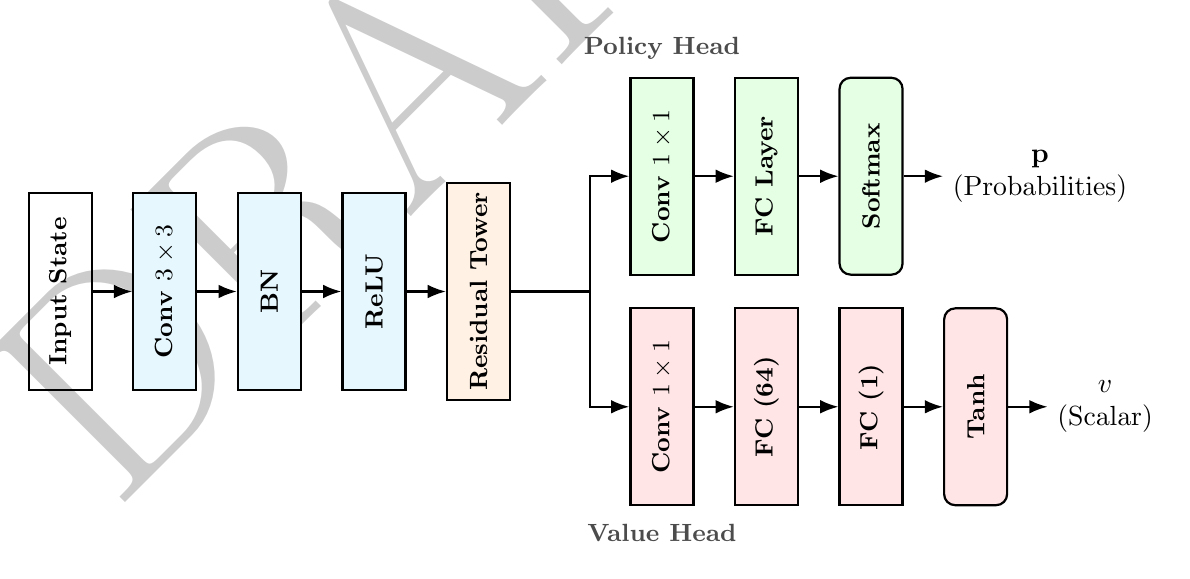
\begin{tikzpicture}[
            node distance=0.8cm and 1.2cm,
            block/.style={draw, rectangle, minimum height=2.5cm, minimum width=.8cm, align=center, font=\small,line width=0.8pt},
            arrow/.style={-{Latex}, thick}
        ]
    
        \node[block] (input) {\rotatebox{90}{\textbf{Input State}}};
        \node[block, right=.5cm of input, fill=cyan!10] (conv1) {\rotatebox{90}{\textbf{Conv $3\times3$}}};
        \node[block, right=.5cm of conv1, fill=cyan!10] (BN) {\rotatebox{90}{\textbf{BN}}};
        \node[block, right=.5cm of BN, fill=cyan!10] (ReLU) {\rotatebox{90}{\textbf{ReLU}}};
        \node[block, right=.5cm of ReLU, fill=orange!10] (res) {\rotatebox{90}{\textbf{Residual Tower}}};
        \coordinate[right=1cm of res] (split);
    
        \node[block, above right=0.2cm and 0.5cm of split, fill=green!10] (p_conv) {\rotatebox{90}{\textbf{Conv $1\times1$}}};
        \node[block, right=.5cm of p_conv, fill=green!10] (p_fc) {\rotatebox{90}{\textbf{FC Layer}}};
        \node[block, right=.5cm of p_fc, fill=green!10, rounded corners] (softmax) {\rotatebox{90}{\textbf{Softmax}}};
        \node[right=0.5cm of softmax, align=center] (p_out) {$\mathbf{p}$\\ (Probabilities)};
    
        \node[block, below right=0.2cm and 0.5cm of split, fill=red!10] (v_conv) {\rotatebox{90}{\textbf{Conv $1\times1$}}};
        \node[block, right=.5cm of v_conv, fill=red!10] (v_fc1) {\rotatebox{90}{\textbf{FC (64)}}};
        \node[block, right=.5cm of v_fc1, fill=red!10] (v_fc2) {\rotatebox{90}{\textbf{FC (1)}}};
        \node[block, right=.5cm of v_fc2, fill=red!10, rounded corners] (tanh) {\rotatebox{90}{\textbf{Tanh}}};
        \node[right=0.5cm of tanh, align=center] (v_out) {$v$\\ (Scalar)};
    
        \draw[arrow] (input) -- (conv1);
        \draw[arrow] (conv1) -- (BN);
        \draw[arrow] (BN) -- (ReLU);
        \draw[arrow] (ReLU) -- (res);
        \draw[thick] (res) -- (split);
        
        \draw[arrow] (split) |- (p_conv);
        \draw[arrow] (p_conv) -- (p_fc);
        \draw[arrow] (p_fc) -- (softmax);
        \draw[arrow] (softmax) -- (p_out);
    
        \draw[arrow] (split) |- (v_conv);
        \draw[arrow] (v_conv) -- (v_fc1);
        \draw[arrow] (v_fc1) -- (v_fc2);
        \draw[arrow] (v_fc2) -- (tanh);
        \draw[arrow] (tanh) -- (v_out);
    
        \node[above=0.1cm of p_conv, font=\bfseries\small, color=black!70] {Policy Head};
        \node[below=0.1cm of v_conv, font=\bfseries\small, color=black!70] {Value Head};
    
        \end{tikzpicture}
        \caption{Architecture of the Policy-Value Network used in AlphaZero.}
    \end{figure}

    The input layer accepts a feature tensor of dimensions $4\times8\times8$, which first passes through a convolutional layer with 64 filters for preliminary feature extraction, equipped with Batch Normalization and ReLU activation functions. Following this, the data flows through a "trunk" network composed of multiple Residual Blocks. Each residual block contains two $3\times3$ convolutional layers and a skip connection. This structure effectively mitigates the vanishing gradient problem in deep networks, enabling the model to capture complex spatial dependencies and long-range stone patterns on the board.

    After the residual tower, the network splits into two independent output heads. The first is the \textbf{Policy Head}, which reduces channel dimensions via a $1\times1$ convolutional layer, flattens the output, and connects to a fully connected layer. Finally, it uses a Softmax activation function to output a probability distribution vector $\mathbf{p}$ of length 64, representing the prior probability of placing a stone at each position on the board. The second is the \textbf{Value Head}, which similarly undergoes dimensionality reduction via a $1\times1$ convolutional layer, connects to a hidden layer with 64 neurons, and finally outputs a scalar $v$ in the interval $[-1, 1]]$ through a fully connected layer with a Tanh activation function. This value assesses the favorability of the current position for the current player. This design, featuring a shared backbone and bifurcated outputs, not only reduces computational cost but also enhances the robustness of feature representation through multi-task learning, leveraging the correlation between policy and value tasks.

    \subsection{Monte Carlo Tree Search (MCTS)}

    Monte Carlo Tree Search (MCTS) is a heuristic search algorithm that evaluates action values by constructing an asymmetric decision tree within the search space. In the AlphaZero framework, MCTS serves as a Policy Improvement operator. Unlike traditional MCTS, the algorithm employed in this study does not rely on random rollouts to evaluate leaf nodes; instead, it utilizes a deep neural network for evaluation. Each node $s$ in the search tree stores statistical information for each edge (action $a$): the visit count $N(s,a)$, the mean action value $Q(s,a)$, and the prior probability $P(s,a)$ provided by the policy network. A complete MCTS simulation consists of the following four steps:

    \begin{figure}[t]
        \centering
        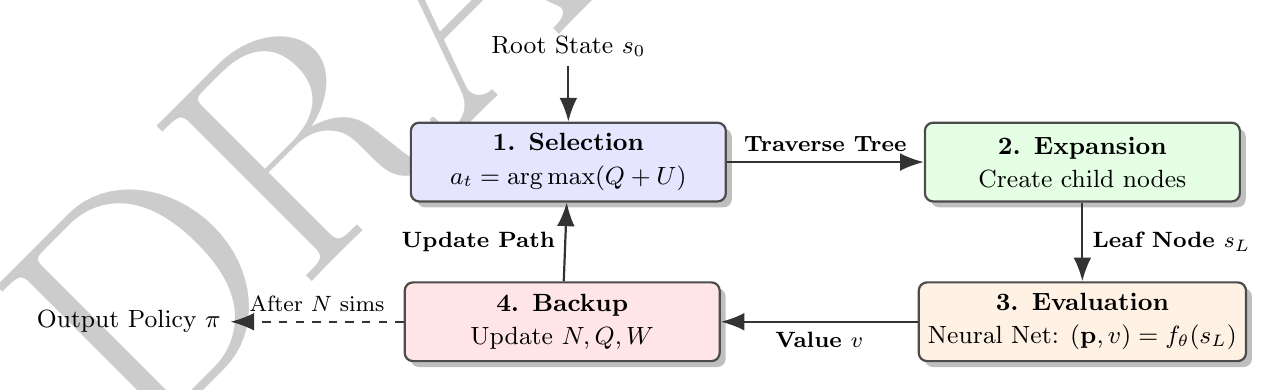
\begin{tikzpicture}[
            node distance=1.5cm and 2cm,
            box/.style={rectangle,  draw=black!70,  thick, fill=white, minimum width=4cm, minimum height=1cm, align=center, rounded corners=3pt,drop shadow},
            arrow/.style={-{Latex[length=3mm]}, thick, draw=black!80},
            label/.style={font=\footnotesize\bfseries}
        ]
    
        \node[box, fill=blue!10] (select) {\small \textbf{1. Selection} \\ \small $a_t = \arg\max(Q + U)$};
        \node[box, fill=green!10, right=2.5cm of select] (expand) {\small \textbf{2. Expansion} \\ \small Create child nodes};
        \node[box, fill=orange!10, below=1cm of expand] (eval) {\small \textbf{3. Evaluation} \\ \small Neural Net: $(\mathbf{p}, v) = f_\theta(s_L)$};
        \node[box, fill=red!10, left=2.5cm of eval] (backup) {\small \textbf{4. Backup} \\ \small Update $N, Q, W$};
    
        \node[inner sep=0pt] (center) at ($(select)!0.5!(eval)$) {};
        
        \draw[arrow] (select) -- node[above, label] {Traverse Tree} (expand);
        \draw[arrow] (expand) -- node[right, label] {Leaf Node $s_L$} (eval);
        \draw[arrow] (eval) -- node[below, label] {Value $v$} (backup);
        \draw[arrow] (backup) -- node[left, label] {Update Path} (select);
    
        \node[above=.7cm of select, align=center] (root) {\small Root State $s_0$};
        \draw[arrow] (root) -- (select);
        
        \node[left=2.2cm of backup, align=center] (pi) {\small Output Policy $\pi$};
        \draw[arrow, dashed] (backup) -- node[above, font=\footnotesize] {After $N$ sims} (pi);
    
        \end{tikzpicture}
        \caption{The Cycle of Monte Carlo Tree Search in AlphaZero}
    \end{figure}

    \subsubsection{Selection}

    A simulation always begins at the root node $s_0$ of the search tree. At each time step $t$, the algorithm selects an action $a_t$ based on a specific selection strategy and descends to the child node $s_{t+1}$ until a leaf node that has not been expanded is reached. To balance exploitation (selecting actions with currently high values) and exploration (trying actions with fewer visits), we adopt the PUCT algorithm based on the Upper Confidence Bound. The rule for selecting action $a$ at node $s$ is as follows:

    \vspace{-.5em}
    \begin{equation}
        a_t=\arg\max\limits_{a}(Q(s,a)+U(s,a))
    \end{equation}

    where $Q(s,a)$ is the current mean value estimate of the action, and $U(s,a)$ is the exploration term, defined as:

    \vspace{-.5em}
    \begin{equation}
        U(s,a)=c_{puct}\cdot P(s,a)\cdot \frac{\sqrt{\sum_bN(s,b)}}{1+N(s,a)}
    \end{equation}

    Here, $P(s,a)$ is the prior probability output by the neural network, and $c_{puct}$ is a hyperparameter controlling the degree of exploration. This formula implies that an action with a high prior probability $P$ and a low visit count $N$ will receive a higher exploration bonus. As the visit count increases, the exploration term gradually decays, and the search becomes increasingly dominated by the actual value $Q$.

    \subsubsection{Expansion}

    When the selection phase reaches a leaf node $s_L$ that does not yet exist in the search tree, it must be expanded. If $s_L$ is a terminal state (i.e., the game has been won, lost, or drawn), the process proceeds directly to the backup step. Otherwise, the algorithm inputs the feature vector of the current state $s_L$ into the policy-value network $f_\theta$.

    The network outputs a probability distribution $\mathbf{p}$ over all legal actions and a state value $v$. At this point, a new node is created for $s_L$ in the search tree, and the probabilities $\mathbf{p}$ are assigned to the prior probabilities $P(s_L,a)$ of the edges emanating from this node. Simultaneously, the visit counts $N(s_L,a)$ and action values $Q(s_L,a)$ for all actions at this node are initialized to zero. In this way, the "intuition" of the neural network is embedded into the growth process of the search tree.

    \subsubsection{Evaluation}

    In traditional MCTS, evaluation is typically achieved by performing random rollouts from the leaf node until the end of the game. However, this method suffers from high variance and computational cost. In our algorithm, we utilize the Value Head of the neural network to directly evaluate the leaf node.

    During the expansion step, the scalar value $v\in[-1,1]$ output by the network $f_\theta(s_L)$ represents the evaluation of the current position $s_L$. This value predicts the expected win rate from the perspective of the current player (+1 for a win, -1 for a loss). This estimated value $v$ replaces the result of traditional random rollouts and serves as the signal for subsequent backpropagation. The advantage of this approach lies in its ability to leverage abstract features learned by the deep network to accurately judge the situation without searching to the very end of the game.

    \subsubsection{Backup}

    Once the valuation $v$ of the leaf node is computed by the neural network, the backup process is initiated. This procedure traverses the search path generated during the selection phase in a bottom-up manner, aiming to integrate the newly acquired state information into the statistics of every node $s$ and corresponding action $a$ along the trajectory. First, to track the frequency of exploration, the visit count for all edges on the path is incremented by 1, denoted as

    \vspace{-.5em}
    \begin{equation}
        N(s,a) \leftarrow N(s,a) + 1
    \end{equation}

    Second, and more critically, the mean action value $Q(s,a)$ is updated using the incremental mean formula

    \vspace{-.5em}
    \begin{equation}
        Q(s,a) \leftarrow Q(s,a)+\frac{v-Q(s,a)}{N(s,a)}
    \end{equation}

    which allows the estimate to dynamically converge towards the true expected return as simulations progress. It is important to note that, due to the zero-sum nature of Gomoku, parent and child nodes represent opposing players. Consequently, during backpropagation, the sign of the value $v$ must be inverted (e.g., using $-v$) at each hierarchical level to ensure that the $Q$ value consistently reflects the winning expectation from the perspective of the player at the current node. Upon completion of the predetermined number of simulations, the accumulated visit statistics at the root node ultimately translate into an improved policy distribution $\pi$, which guides the actual move decision in the game.
    
	\section{Experiments}

    This experiment aims to validate the effectiveness of the AlphaZero algorithm in an $8\times8$ Freestyle Gomoku environment. The entire training process strictly follows the "Self-Play" strategy, where the agent relies solely on games played against historical versions of itself to generate training samples, without any dependency on human expert data. To ensure training stability and diversity in data distribution, we established an Experience Replay Buffer with a capacity of 10,000. During each training step, 512 data points (Batch Size) are randomly sampled from the buffer to update the neural network parameters using the Adam optimizer with a learning rate of $2\times10^{-3}$. In the data collection phase, the number of MCTS simulations ($n_{playout}$) per move is set to 400, and the exploration constant $c_{puct}$ is set to 5 to balance exploration and exploitation during the search. Furthermore, leveraging the rotational invariance and symmetry of the Gomoku board, we augmented the data by rotating and flipping the board states before storing them in the buffer, effectively expanding the sample size by a factor of eight and significantly improving sample efficiency.

    \begin{figure}[t]
        \centering
        \begin{minipage}{.48\textwidth}
            \centering
            \includegraphics[width=\textwidth]{figure/loss_curve.png}
            \caption{Loss Curve of the Training Process}
        \end{minipage}
        \begin{minipage}{.48\textwidth}
            \centering
            \includegraphics[width=\textwidth]{figure/win_rate_curve.png}
            \caption{Win Rate Curve in Validation Phase}
        \end{minipage}
    \end{figure}

    The trend of the loss function during training is shown in the figure. In the initial stage (the first 200 batches), the loss value dropped rapidly from approximately 4.5 to 3.5, indicating that the neural network quickly grasped the basic rules of Gomoku, the legality of moves, and preliminary positional judgment. Subsequently, the curve exhibited an oscillating downward trend, eventually stabilizing around 2.75 by the 1200th batch. It is worth noting that such oscillation is reasonable in self-play-based reinforcement learning: as the agent's playing strength continuously improves, the distribution of games generated by self-play (Data Distribution) constantly shifts. This causes the optimization target (Target Policy) of the neural network to be dynamic, yet this phenomenon did not hinder the overall convergence of the policy.
    
    To quantitatively evaluate the agent's combat performance, we conducted a benchmark test on the current model every 50 batches. The evaluation opponent was an agent based on Pure Monte Carlo Tree Search (Pure MCTS). To increase the difficulty and persuasiveness of the evaluation, we set the simulation count for this baseline agent to 1000, which is significantly higher than the 400 simulations used during training. In the evaluation games, the AlphaZero agent played as Black, while the baseline agent played as White. To eliminate the influence of first-move advantage, we adopted an alternating verification strategy where "our agent moves first in odd-numbered games, and the opponent moves first in even-numbered games." The win rate curve, as shown in the figure, reveals that in the first 400 batches, AlphaZero and Pure MCTS were evenly matched, with the win rate fluctuating between 0.4 and 0.7, indicating an exploratory learning phase. However, starting from the 400th batch, the win rate showed explosive growth, rapidly breaking through 0.9. After 700 batches, AlphaZero maintained a nearly 100\% win rate against the Pure MCTS agent despite the latter's higher search count, strongly proving that the neural network had acquired positional evaluation capabilities far superior to mere brute-force search.
    
    The evolution of the game boards further intuitively demonstrates the progression of AlphaZero's strategy. In the evaluation at the 100th batch (early validation stage), Black's (AlphaZero) moves were relatively scattered and lacked obvious coherence, often relying on opponent errors or luck to win, resulting in disorganized game patterns. By the 700th batch (mid-validation stage), Black had learned to construct continuous attack formations, identify critical defensive points, and quickly form "four-in-a-row" threats to force White into passive defense, corresponding to a significant increase in win rate. By the 1300th batch (late validation stage), the agent displayed superb tactical literacy, capable of utilizing advanced techniques such as "double-three" and "traps" to end the game in very few turns. As shown in the final game board, Black demonstrated extreme aggression from the opening, pressing step by step with precise moves, leaving White (Pure MCTS) with no escape within a dozen moves.

    \begin{figure}
        \begin{minipage}{\textwidth}
            \centering
            \includegraphics[width=.9\textwidth]{figure/eval_batch_100.png}
            \caption{Game Record for Verification Stage (Batch=100)}
        \end{minipage}
        
        \vspace{2em}
        
        \begin{minipage}{\textwidth}
            \centering
            \includegraphics[width=.9\textwidth]{figure/eval_batch_700.png}
            \caption{Game Record for Verification Stage (Batch=700)}
        \end{minipage}
        
        \vspace{2em}
        
        \begin{minipage}{\textwidth}
            \centering
            \includegraphics[width=.9\textwidth]{figure/eval_batch_1300.png}
            \caption{Game Record for Verification Stage (Batch=1300)}
        \end{minipage}
    \end{figure}

    Finally, there is an interesting anecdote worth mentioning that serves as a qualitative evaluation. My fiancée is quite proficient at Gomoku; in fact, I have historically never managed to win a single game against her. After completing the training and implementing a graphical user interface, I invited her to play against the trained agent. The results were striking: the agent achieved a dominant victory, and she barely won any matches. Although it is regrettable that I did not record the specific game logs (kifu) of these matches, this outcome strongly demonstrates that the agent has effectively mastered advanced strategies through self-play. It further validates the immense advantages of deep reinforcement learning in feature extraction and long-term planning. On a more personal and humorous note, I was finally able to "avenge" my past defeats against her, albeit with the assistance of the AI.
	
	\section{Conclusion}
	
	By constructing and training an agent based on the AlphaZero architecture, this project strongly validates the universality and efficiency of deep reinforcement learning in the domain of perfect information games. The experimental results demonstrate that without any intervention of human expert knowledge (such as opening books, game records, or handcrafted features), the agent can rapidly master advanced Gomoku tactics solely through self-play, achieving a landslide victory against a Pure Monte Carlo Tree Search (Pure MCTS) baseline. This conclusion highlights the immense potential of combining "neural network intuition" with "tree search logic": the neural network utilizes its generalization capabilities to significantly prune the search space, while MCTS provides robust policy improvement targets for the network. This virtuous cycle enables the algorithm to overcome the performance bottlenecks of traditional search algorithms under limited computational resources.

    Although this study has achieved satisfactory results on an $8\times8$ board, there remains ample room for exploration to fully solve the standard Gomoku problem. Future work will focus on three main directions: First, expansion of the state space. We intend to migrate the algorithm to the standard $15\times15$ board, which will impose higher demands on the neural network's feature extraction capabilities and convergence speed. Second, refinement of game rules. To align with real-world competitive scenarios, we need to introduce "forbidden moves" (such as the double-three and double-four restrictions) into the environment model, which will significantly increase the complexity of the game tree and logic judgment. Finally, optimization of computational efficiency. Given that the serial simulation nature of MCTS limits training speed, future iterations could incorporate parallel tree search algorithms based on Virtual Loss to fully leverage multi-core CPU or GPU resources, thereby accelerating the evolution of the agent.

    \section{Postscript}

    Time flies, and recently I have felt the physical toll of a demanding schedule. Regarding this assignment, I labored under the misconception that the deadline was December 9th, only to realize on December 5th that it was actually due on December 3rd.

    Over the past month, I have been continuously dedicating myself to iterating on my project and debugging. Concurrently, my fiancée and I have been occupied with our pre-marital arrangements, alongside arranging her internship and housing for the coming semester. Furthermore, I undertook a work-study position at the college to assist in auditing faculty research performance. The convergence of these multiple responsibilities led to my confusion regarding the deadline. I am deeply sorry and regretful for this oversight. I write this postscript to explain the circumstances and sincerely hope that the high quality of this report will serve to make amends for the late submission.
	
	\let\cleardoublepage\clearpage
	
	\begin{thebibliography}{99}  
		\bibitem{ref1} 董豪, 丁子涵, 仉尚航等. 深度强化学习: 基础、研究与应用[M]. 第1版. 北京:电子工业出版社, 2021.
        \bibitem{ref10} 搜狗百科. 人机围棋大战[EB/OL]. [2025-12-09]. https://baike.sogou.com/m/fullLemma?lid=1\ 31584116.
        \bibitem{ref2} 张伟楠, 沈键, 俞勇. 动手学强化学习[M]. 第1版. 北京:人民邮电出版社, 2022.
        \bibitem{ref3} 赵世钰. 强化学习的数学原理[M]. 第1版. 北京:清华大学出版社, 2025.
        \bibitem{ref4} 赵世钰. 强化学习的数学原理:英文[M]. 第1版. 北京:清华大学出版社, 2024.
        \bibitem{ref5} Kocsis L, Szepesvári C. Bandit based monte-carlo planning[C]//European conference on machine learning. Berlin, Heidelberg: Springer Berlin Heidelberg, 2006: 282-293.
        \bibitem{ref6} Mnih V, Kavukcuoglu K, Silver D, et al. Human-level control through deep reinforcement learning[J]. nature, 2015, 518(7540): 529-533.
        \bibitem{ref7} Silver D, Huang A, Maddison C J, et al. Mastering the game of Go with deep neural networks and tree search[J]. nature, 2016, 529(7587): 484-489.
        \bibitem{ref8} Silver D, Hubert T, Schrittwieser J, et al. A general reinforcement learning algorithm that masters chess, shogi, and Go through self-play[J]. Science, 2018, 362(6419): 1140-1144.
        \bibitem{ref9} Silver D, Schrittwieser J, Simonyan K, et al. Mastering the game of go without human knowledge[J]. nature, 2017, 550(7676): 354-359.
	\end{thebibliography}
    
\end{document}
